\documentclass[conference]{IEEEtran}
\usepackage{cite}
\usepackage{graphicx}
\usepackage{amsmath,amssymb,amsfonts}
\usepackage{algorithmic}
\usepackage{textcomp}
\usepackage{float}
\usepackage{xcolor}
\usepackage{tabularx}

\title{Weed Detection Using Custom Object Detection Models and Embedded Deployment on Raspberry Pi}

\author{
    \IEEEauthorblockN{Christopher Arredondo}
    \IEEEauthorblockA{\textit{Costa Rica Institute of Technology} \\
    Email: chrisarrefal@estudiantec.cr}
}

\begin{document}

\maketitle

\begin{abstract}
Weed detection is a challenging problem due to the visual similarity between weeds and surrounding vegetation, such as grass. This project explores the development of a custom object detection model trained from scratch to identify weeds in images. The model leverages a dataset annotated with bounding boxes and undergoes multiple iterations to improve performance. The final system is deployed on a Raspberry Pi 4 using TensorFlow Lite for real-time inference, showcasing its feasibility for residential applications such as tracking weeds in a lawn. This work highlights the challenges of weed detection, including color and texture similarity, and discusses potential improvements using prebuilt models such as YOLO. The proposed solution demonstrates the practicality of a lightweight, custom model for edge-device deployment.
\end{abstract}

\begin{IEEEkeywords}
Weed detection, object detection, convolutional neural networks, TensorFlow Lite, Raspberry Pi, machine learning.
\end{IEEEkeywords}

\section{Introduction}
\IEEEPARstart{W}{eed} detection is a common problem, particularly in environments such as residential lawns, where weeds compete with grass for nutrients, sunlight, and water. Left unmanaged, weeds can diminish the aesthetic value and health of a lawn. However, manually identifying and removing weeds is labor-intensive and prone to inefficiencies, especially when weeds visually resemble grass in terms of color and texture. These similarities make automated detection a challenging task.

This project focuses on developing a custom object detection model for identifying weeds in images. Unlike prebuilt models, which rely on transfer learning and pretraining on large datasets, the proposed solution was trained from scratch using a dataset annotated in Pascal VOC format. The model underwent several iterations to improve performance, including enhancements in architecture and training strategies.

A key motivation for this work is its potential application in residential settings. By deploying the trained model on a Raspberry Pi 4 using TensorFlow Lite, the system enables real-time weed tracking and management in a home lawn. Such a system can provide year-round monitoring, offering a practical and efficient alternative to traditional methods of weed control.

This paper details the challenges of weed detection, the iterative development of the model, and the feasibility of deploying the system on embedded hardware for real-world applications. It also discusses the potential benefits of integrating prebuilt object detection models, such as YOLO, to further enhance performance.



\section{Theoretical Framework}
\subsection{Overview of Object Detection}
Object detection is a computer vision task that involves identifying and localizing objects within an image. Unlike image classification, which assigns a single label to an entire image, object detection predicts both the category of objects and their locations using bounding boxes. The task is essential in applications such as autonomous vehicles, surveillance, and agricultural monitoring, where identifying objects and their spatial relationships is crucial.

Modern object detection systems are typically based on deep learning architectures, particularly Convolutional Neural Networks (CNNs), which are great at extracting hierarchical features from images \cite{subeesh2022deep}. Object detection models are broadly classified into two categories:
\begin{itemize}
    \item \textbf{Two-Stage Detectors:} These models, such as Faster R-CNN, first generate region proposals and then classify them into object categories. While accurate, they are computationally expensive and less suited for real-time applications.
    \item \textbf{Single-Stage Detectors:} Models like YOLO and SSD (Single Shot Multibox Detector) perform detection and classification in a single pass, offering a trade-off between speed and accuracy \cite{rai2024weedvision}.
\end{itemize}

\subsection{State of the Art and Initial algorithms in Object Detection}
The current state-of-the-art object detection models leverage advances in CNNs, feature pyramids, attention mechanisms, and transformer-based architectures to improve accuracy and speed. Each model introduces unique innovations to address various challenges in object detection.

\begin{itemize}
    \item \textbf{Faster R-CNN:} A two-stage detector that introduced the concept of Region Proposal Networks (RPNs), enabling end-to-end object detection pipelines. Faster R-CNN excels in accuracy by employing a deep convolutional backbone for feature extraction, followed by region-specific feature classification and bounding box regression \cite{ren2015faster}. However, the two-stage process limits its real-time applicability in embedded environments, as it prioritizes accuracy over speed.
    
    \item \textbf{YOLO (You Only Look Once):} Initially proposed by Redmon et al. \cite{redmon2016yolo}, YOLO is a single-stage object detector that frames detection as a regression problem. Unlike traditional two-stage detectors, YOLO predicts bounding boxes and class probabilities directly from the input image in one forward pass. This simplicity enables real-time performance, making YOLO ideal for applications where speed is critical, such as autonomous driving, drone navigation, and edge computing.

    Over the years, YOLO has evolved significantly with iterations like YOLOv4, YOLOv5, YOLOv7, and the most recent YOLOv11. YOLOv11 introduces architectural innovations, including:
    \begin{itemize}
        \item \textbf{C3k2 Blocks:} Enhancements to cross-stage partial blocks for better feature fusion.
        \item \textbf{SPPF (Spatial Pyramid Pooling - Fast):} A faster and more efficient spatial pyramid pooling module for capturing multi-scale information.
        \item \textbf{C2PSA (Convolutional Block with Parallel Spatial Attention):} Improved spatial attention mechanisms that enhance the model’s ability to focus on relevant regions in complex images.
    \end{itemize}
    These advancements make YOLOv11 significantly more robust and accurate, with variants ranging from nano to extra-large models, catering to a diverse set of applications from embedded systems to high-performance computing \cite{khanam2024yolov11}.
    
    \item \textbf{EfficientDet:} This model leverages compound scaling and neural architecture search to optimize both speed and accuracy. EfficientDet uses a BiFPN (Bidirectional Feature Pyramid Network) for efficient multi-scale feature fusion and introduces compound scaling to uniformly scale the depth, width, and resolution of the network \cite{tan2020efficientdet}. Its design strikes a balance between computational efficiency and detection performance, making it suitable for resource-constrained scenarios.
    
    \item \textbf{Co-DETR:} Combining convolutional backbones with transformer-based decoders, Co-DETR extends the capabilities of detection transformers. It employs a CNN backbone for initial feature extraction and a transformer decoder to capture long-range dependencies \cite{zong2022code}. By integrating feature pyramids, Co-DETR effectively handles multi-scale object detection, achieving state-of-the-art performance on benchmark datasets like MS COCO while maintaining computational efficiency.
\end{itemize}

These models represent different ways of tackling the challenges of object detection. While two-stage detectors like Faster R-CNN prioritize accuracy, single-stage models such as YOLO and EfficientDet offer a balance between speed and precision. Transformer-based models like Co-DETR highlight the growing trend of integrating attention mechanisms and advanced feature pyramids for improved performance across across multiple domains. The recent advancements in YOLOv11 further demonstrate how architectural innovations can make object detection more accessible across varying hardware constraints, including edge devices.

\section{Methodology}

This section describes the workflow for developing the weed detection model, including dataset preparation, model architecture design, training, evaluation, and deployment on an embedded system. 

\subsection{Dataset Preparation}
Two datasets were used during the development phase:
\begin{itemize}
    \item \textbf{Manually Captured Images:} Initially, 300 images of weeds in a lawn were captured using a smartphone. These images were annotated manually using LabelImg, a tool for bounding box annotation in Pascal VOC format. While the dataset provided a starting point for model training, its size was insufficient for achieving high accuracy, as it lacked sufficient diversity and quantity.
    \item \textbf{Roboflow Dataset:} To address the limitations of the manually captured dataset, a publicly available dataset containing 4,203 annotated images of weeds was sourced from Roboflow \cite{ahmed2024imageweed}. Images in this dataset were consistent in resolution (640x640) and included bounding box annotations in Pascal VOC format, facilitating seamless integration into the training pipeline.
\end{itemize}

Data augmentation techniques were applied to increase dataset diversity, including random rotations, horizontal and vertical flips, brightness adjustments, and cropping. These techniques were essential to enhance the model's generalization capabilities.

\subsection{Model Design and Iterations}
The custom object detection model was iteratively designed and improved over three main versions. Each iteration addressed shortcomings observed during training and evaluation:

\subsubsection{Baseline Model}
The initial model consisted of two convolutional layers followed by a fully connected layer for bounding box prediction. While computationally lightweight, the model suffered from high training loss and poor convergence due to inadequate feature extraction capacity.

\subsubsection{Enhanced CNN}
The second version introduced an additional convolutional layer and max-pooling operations to improve feature extraction and spatial hierarchy learning. Batch normalization layers were added to stabilize training. However, overfitting became evident due to the relatively small dataset size, necessitating data augmentation to improve generalization.

\subsubsection{Final Model}
The final model incorporated four convolutional layers with increased filter sizes for deeper feature extraction. Batch normalization and dropout layers were added to mitigate overfitting, and the fully connected layer was expanded to enhance the model's capacity for learning complex patterns. Table \ref{tab:model_architecture} summarizes the architectural evolution across iterations.

\subsection{Training Process}
The model was trained from scratch using the TensorFlow/Keras framework on a workstation with the following specifications:
\begin{itemize}
    \item \textbf{Processor:} Intel(R) Core(TM) i5-10600K CPU @ 4.10GHz
    \item \textbf{RAM:} 48 GB
    \item \textbf{Operating System:} Ubuntu 20.04 under Windows 11 (via WSL)
    \item \textbf{GPU:} NVIDIA RTX 3080 with 10GB VRAM
\end{itemize}

Training hyperparameters included:
\begin{itemize}
    \item Optimizer: Adam
    \item Learning rate: 0.001
    \item Loss function: Mean Squared Error (MSE)
    \item Batch size: 10
    \item Epochs: 50
\end{itemize}

While the final model achieved moderate accuracy (0.41) after 50 epochs, further improvements may be possible with extended training and hyperparameter tuning.

\subsection{Evaluation and Results}
The trained model was evaluated on the test set, and performance was measured using accuracy and loss metrics. Qualitative results are shown in Section VI, where ground truth bounding boxes are compared with model predictions. While the model performed reasonably well, it struggled to differentiate weeds from visually similar elements like grass in certain cases (e.g., Figure \ref{fig:result4}).

\subsection{YOLO-Based Model Comparison}
To benchmark the custom model, a simplified YOLO-based architecture was implemented and trained using the same dataset. The details regarding this model will be discussed later in this paper.

\subsection{Deployment on Raspberry Pi 4}
The final model was converted into a TensorFlow Lite format for deployment on a Raspberry Pi 4, an affordable embedded platform suitable for real-time applications. Quantization techniques were applied during conversion to reduce model size and improve inference speed.

The deployed system processes images in real time, detecting weeds in residential lawns and highlighting them with bounding boxes. This embedded implementation demonstrates the practicality of using lightweight custom models for weed detection in edge environments.



\section{Deep Learning Models for Weed Detection}
Deep learning models, particularly Convolutional Neural Networks (CNNs), have revolutionized image analysis tasks by enabling automated feature extraction. CNNs consist of convolutional layers, pooling layers, and fully connected layers, which work together to learn spatial hierarchies and patterns in data \cite{subeesh2022deep}.

In this study, a custom CNN model was designed, trained from scratch, and optimized for weed detection. While pre-trained models such as InceptionV3 and YOLO offer high accuracy and efficiency, their use was avoided to adhere to project constraints. The architecture iteratively improved from a baseline model with two convolutional layers to a final version featuring four convolutional layers with batch normalization and data augmentation to prevent overfitting.

Past studies have explored similar architectures for agricultural applications. For example, Rai and Sun \cite{rai2024weedvision} proposed a single-stage architecture that combines object detection and instance segmentation for drone-acquired images, achieving high precision in bounding-box detection. Similarly, Subeesh et al. \cite{subeesh2022deep} demonstrated the effectiveness of InceptionV3 for detecting weeds in polyhouse-grown bell peppers, highlighting the role of architecture depth and data preprocessing in enhancing performance.

\section{Model Development}
The design and optimization of the weed detection model involved multiple iterations, with incremental improvements in architecture and training strategies. Each iteration aimed to address the limitations observed in the previous versions.

\subsection{Model Architecture Summary}
Table \ref{tab:model_architecture} summarizes the layers used in each iteration of the model, illustrating the progression of architectural complexity.

\begin{table}[H]
\centering
\caption{Model Architecture Summary Across Iterations}
\label{tab:model_architecture}
\begin{tabularx}{\columnwidth}{|l|X|X|X|}
\hline
\textbf{Layer Type}       & \textbf{Baseline} & \textbf{Enhanced CNN} & \textbf{Final Model} \\ \hline
Input Layer               & 640x640x3         & 640x640x3             & 640x640x3           \\ \hline
Conv2D (Filters, Kernel)  & (32, 3x3)         & (64, 3x3)             & (128, 3x3)          \\ \hline
Conv2D (Filters, Kernel)  & (64, 3x3)         & (128, 3x3)            & (64, 3x3)           \\ \hline
Conv2D (Filters, Kernel)  & -                 & (64, 3x3)             & (32, 3x3)           \\ \hline
MaxPooling2D              & -                 & Yes                   & Yes                 \\ \hline
Batch Normalization       & -                 & No                    & Yes                 \\ \hline
Flatten                   & Yes               & Yes                   & Yes                 \\ \hline
Dense Layers              & (64)              & (128)                 & (64, 128)           \\ \hline
Output Layer              & 4xBounding Boxes  & 4xBounding Boxes      & 4xBounding Boxes    \\ \hline
\end{tabularx}
\end{table}



\section{Challenges in Weed Detection}
Weed detection presents unique challenges due to the visual similarity between weeds and crops or surrounding vegetation, such as grass. These similarities often result in false positives or missed detections, as demonstrated in Figure \ref{fig:result4}, where the model incorrectly identifies non-weed regions as weeds.

Moreover, varying environmental factors such as lighting conditions, occlusions, and overlapping vegetation add to the complexity of detection. Manual annotation of datasets further complicates the development process. In this project, the initial dataset of 300 manually annotated images proved insufficient for training, necessitating the use of a larger dataset from Roboflow \cite{ahmed2024imageweed}.

\section{Results}
The results showcase both the capabilities and limitations of the final model. Figures \ref{fig:result1}, \ref{fig:result2}, and \ref{fig:result3} present examples of successful predictions, while Figure \ref{fig:result4} highlights a case of model confusion.

\begin{figure}[H]
    \centering
    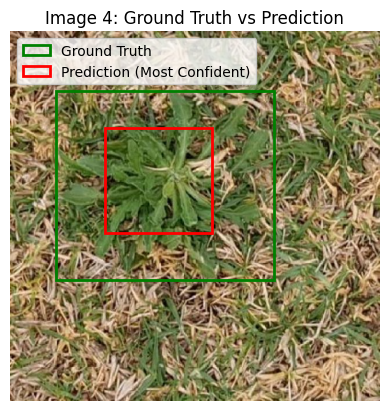
\includegraphics[width=\columnwidth]{result1.png}
    \caption{Ground Truth vs. Prediction: Example 1}
    \label{fig:result1}
\end{figure}

\begin{figure}[H]
    \centering
    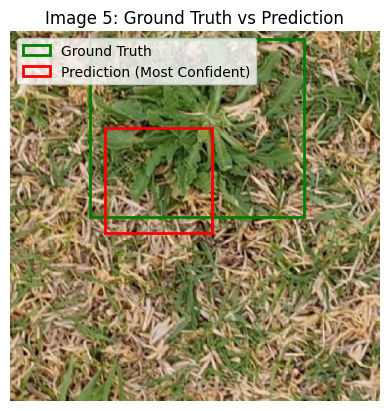
\includegraphics[width=\columnwidth]{result2.png}
    \caption{Ground Truth vs. Prediction: Example 2}
    \label{fig:result2}
\end{figure}

\begin{figure}[H]
    \centering
    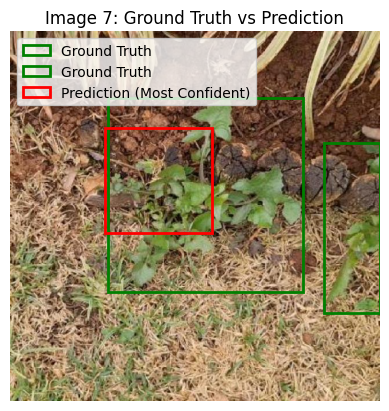
\includegraphics[width=\columnwidth]{result3.png}
    \caption{Ground Truth vs. Prediction: Example 3}
    \label{fig:result3}
\end{figure}

\begin{figure}[H]
    \centering
    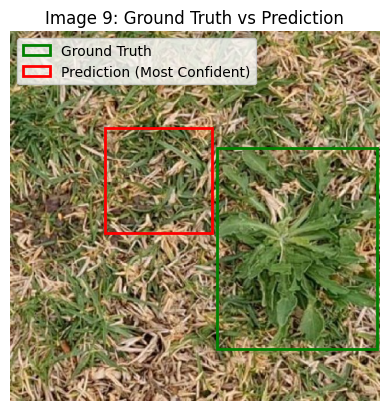
\includegraphics[width=\columnwidth]{result4.png}
    \caption{Model Confusion Example: Incorrectly Detecting Weeds}
    \label{fig:result4}
\end{figure}

The final model achieved an accuracy of 0.41 after 50 epochs. While this demonstrates the model's ability to generalize to some extent, the performance is insufficient for practical deployment. Several factors likely contributed to these results:

\begin{itemize}
    \item \textbf{Limited Architectural Complexity:} The model, while custom-built, lacks the depth and optimization of advanced object detection frameworks like YOLO or Co-DETR. These models incorporate techniques such as anchor boxes, region proposal networks, and multi-scale feature extraction, which enhance object detection capabilities.
    \item \textbf{Dataset Imbalance and Complexity:} The visual similarity between weeds and grass poses a unique challenge, leading to false positives and missed detections.
    \item \textbf{Overfitting and Underfitting:} The model likely suffers from a combination of overfitting during early epochs and underfitting in its later stages, as evidenced by the plateauing validation accuracy and high validation loss.
\end{itemize}

Figure \ref{fig:result4} exemplifies one of the model's key limitations: the incorrect detection of non-weed regions as weeds. This underscores the need for more advanced architectures and richer datasets.

\section{Comparison with YOLO-Based Model}
To evaluate the advantages of prebuilt architectures, a simplified YOLO-based model was implemented and trained for 50 epochs. The architecture consisted of five convolutional blocks with leaky ReLU activation and max pooling, followed by a fully connected layer to predict bounding box coordinates. 

The YOLO-based model achieved significantly higher accuracy compared to the custom model, as seen in table \ref{tab:model_comparison}. Figure \ref{fig:yolo_result1} illustrates one of the YOLO model's predictions.

\begin{figure}[H]
    \centering
    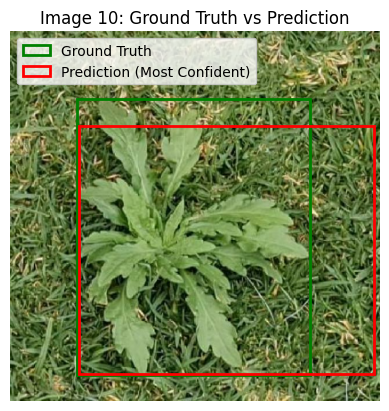
\includegraphics[width=\columnwidth]{result_yolo1.png}
    \caption{YOLO Model: Ground Truth vs. Prediction}
    \label{fig:yolo_result1}
\end{figure}

\begin{table}[H]
    \centering
    \caption{Comparison of YOLO and Custom Model Results After 50 Epochs}
    \label{tab:model_comparison}
    \begin{tabularx}{\columnwidth}{|l|X|X|X|X|}
    \hline
    \textbf{Model}        & \textbf{Epochs} & \textbf{Accuracy} & \textbf{Validation Accuracy} & \textbf{Loss}         \\ \hline
    YOLO-Based Model      & 50              & 0.6954            & 0.5850                       & 0.0861                \\ \hline
    Custom Model          & 50              & 0.4141            & 0.4086                       & 22537                 \\ \hline
    \end{tabularx}
\end{table}

Although the YOLO model's accuracy was higher, the training process was not saturated, suggesting that further improvements could be achieved with additional epochs. This highlights the potential of YOLO-based architectures for weed detection tasks, especially when the computational constraints of embedded systems are relaxed.


\section{Conclusion}
This paper presents a comprehensive approach to weed detection, comparing a custom object detection model with a simplified YOLO-based architecture. While the custom model demonstrated the feasibility of real-time detection on embedded systems, the YOLO model significantly outperformed it, achieving higher accuracy and stability during training. These findings underscore the importance of architectural design in achieving robust object detection performance.

Future work should focus on extending training epochs, enhancing dataset quality, and exploring the integration of advanced YOLO-based features to further improve detection accuracy.

\bibliographystyle{IEEEtran}
\bibliography{references}

\end{document}
